%%=============================================================================
%% Implementatie
%%=============================================================================

\chapter{Implementatie}
\label{ch:implementatie}

Dit hoofdstuk beschrijft in detail de implementatie van RESTful principes en de aanpassingen in de frontend applicatie voor de Bright\-Eats API. We behandelen codevoorbeelden, tools en de gemaakte keuzes.

\section{Inleiding}

In dit hoofdstuk duiken we in de concrete implementatie van de Bright\-Eats API, waarbij we de theoretische principes uit de voorgaande hoofdstukken vertalen naar werkende code. We bouwen voort op de keuzes die gemaakt zijn in de literatuurstudie: de focus ligt op het implementeren van een robuuste RESTful API, ondersteund door een uitgebreide OpenAPI-specificatie, zonder de implementatie van HATEOAS. Verder zullen we, waar relevant, de Zalando RESTful API Guidelines als leidraad gebruiken. Dit hoofdstuk is opgedeeld in drie delen. Eerst behandelen we de implementatie van de backend in Laravel, gevolgd door de ontwikkeling van de frontend in Vue.js. Tenslotte tonen we hoe de OpenAPI-specificatie is geïntegreerd in het ontwikkelproces en hoe deze bijdraagt aan de documentatie, validatie en testing van de API.

\section{BrightEats}

Bright\-Eats is een applicatie die toelaat om lunchbestellingen te plaatsen en te beheren voor werknemers van BrightAnalytics. Gebruikers loggen in en zien vervolgens een lijst van winkels met openstaande groepsbestellingen. Vervolgens kunnen ze een bestelling plaatsen in een groepsbestelling, of zelf een groepsbestelling starten. De hoofdfunctionaliteit en het nut van de applicatie is dat de persoon die de groepsbestelling start, makkelijk betaalverzoeken kan sturen naar de deelnemers van de bestelling. De backend API moet dus in staat zijn om betalingsverzoeken te genereren in de vorm van QR-codes.

\begin{figure}[H]
    \centering
    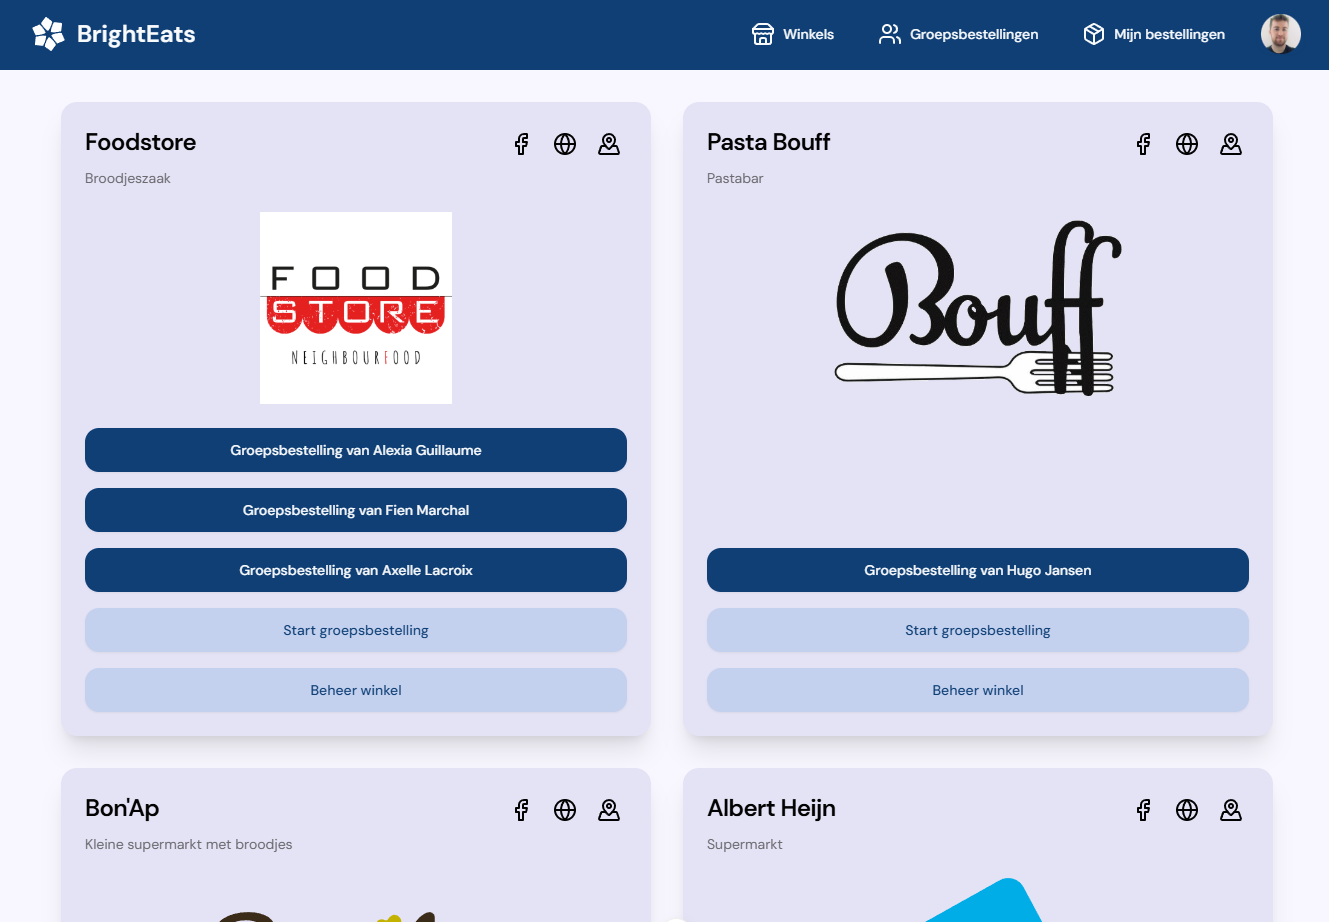
\includegraphics[width=0.8\textwidth]{brighteats.png}
    \caption{De homepage van de BrightEats applicatie.}
    \label{fig:brighteats}
\end{figure}

\begin{figure}[H]
    \centering
    
\includegraphics[width=0.8\textwidth]{brighteats-payment-page.png}
    \caption{De betalingspagina van de BrightEats applicatie, met een QR-code voor de betaling.}
    \label{fig:brighteats-shop}
\end{figure}

\bigskip

Authenticatie gebeurt via Google SSO, waarbij gebruikers inloggen met hun BrightAnalytics Google account. De backend API is verantwoordelijk voor het beheren van gebruikers, winkels, menu's, groepsbestellingen en betalingsverzoeken. De frontend applicatie is verantwoordelijk voor het tonen van deze gegevens en het toelaten van interactie met de gebruiker.

\section{Backend - Algemene aanpak}

De implementatie van de RESTful principes in de Laravel backend van de Bright\-Eats API werd aangepakt met een iteratieve aanpak, waarbij we stapsgewijs verschillende onderdelen van de API ontwikkelden en verfijnden. Hierbij maakten we veel gebruik van Laravel's ingebouwde functionaliteiten, zoals resource controllers en routes, en hielden we ons zo veel mogelijk aan de opgestelde richtlijnen.

\subsection{Architectuur en RESTful principes}

Laravel's architectuur is perfect voor het bouwen van RESTful API's. We maken gebruik van resource controllers om gestructureerd CRUD-operaties (Create, Read, Update, Delete) op onze resources, zoals \texttt{Order}, \texttt{Shop}, \texttt{Item} en \texttt{GroupOrder}, te definiëren. Deze controllers worden gekoppeld aan routes in het \texttt{api.php} bestand, dat dient als het centrale punt voor het definiëren van alle API endpoints.

\subsubsection{Autorisatie}

Voor autorisatie gebruiken we Policies. Zo is er bijvoorbeeld een \texttt{OrderPolicy} die bepaalt welke gebruikers welke acties mogen uitvoeren op een \texttt{Order}.

\subsubsection{Validatie}

Voor validatie gebruiken we specifieke request classes, zoals \texttt{StoreOrderRequest} en \texttt{UpdateOrderRequest}, die de validatieregels voor inkomende requests definiëren.

\subsubsection{Authenticatie}

Authenticatie wordt afgehandeld door Laravel Sanctum. Dit pakket biedt een eenvoudige manier om API tokens te beheren en gebruikers te authenticeren. Voor Bright\-Eats is Google Single Sign-On (SSO) de enige authenticatiemethode. Gebruikers loggen in door een POST request te sturen naar \texttt{/users} met hun Google credential. Het systeem verifieert deze credential en genereert een Sanctum token voor de gebruiker.

\subsubsection{Businesslogica}

De businesslogica bevindt zich voornamelijk in Service classes. Voor orders hebben we bijvoorbeeld de \texttt{OrderService}, \texttt{OrderItemsManager} en \texttt{QrCodeGenerator} classes, die verantwoordelijk zijn voor respectievelijk het beheren van orders, het beheren van order items en het genereren van QR-codes voor betalingen. Models, zoals \texttt{Order}, bevatten eenvoudige berekeningen en methoden, terwijl complexere logica wordt geabstraheerd naar services.

\subsubsection{Datarepresentatie}

Voor het terugsturen van data gebruiken we API Resources. Deze transformeren de models naar een JSON-structuur die geschikt is voor de API. We gebruiken verschillende resources, zoals \texttt{OrderResource}, \texttt{OrderResourceWithItems} en \texttt{OrderResourceWithGroupOrder}, om de nodige data te embedden, afhankelijk van de context.

\section{Beschrijving van de API Routes}

Het \texttt{api.php} bestand definieert alle routes voor de Bright\-Eats API. Hieronder volgt een gedetailleerde beschrijving van elke route, gegroepeerd per resource en functionaliteit. Alle routes, met uitzondering van de inlog-route, vallen onder de \texttt{auth:sanctum} middleware, wat betekent dat gebruikers geauthenticeerd moeten zijn om toegang te krijgen.

\subsection{Authenticatie}

\begin{itemize}
  \item \textbf{POST /users:} Deze route wordt gebruikt voor authenticatie via Google SSO. Gebruikers sturen hun Google credential mee in de request body. Deze credential wordt door de Google API in de frontend ontvangen. Bij succesvolle validatie wordt een Sanctum token gegenereerd en teruggestuurd. Dit is de enige manier om in te loggen in de applicatie.
\end{itemize}

\subsection{Winkels (shops)}

\begin{itemize}
  \item \textbf{GET /shops:} Haalt een lijst op van alle winkels. Dit endpoint geeft per winkel ook alle groepsbestellingen terug die momenteel openstaan.
  \item \textbf{POST /shops:} Maakt een nieuwe winkel aan.
  \item \textbf{GET /shops/{shop}:} Haalt de details van een specifieke winkel op, geïdentificeerd door \texttt{{shop}}.
  \item \textbf{PATCH /shops/{shop}:} Werkt de gegevens van een specifieke winkel bij.
  \item \textbf{DELETE /shops/{shop}:} Verwijdert een specifieke winkel.
  \item \textbf{POST /shops/{shop}/group-orders:} Maakt een nieuwe groepsbestelling aan bij een specifieke winkel.
\end{itemize}

\subsection{Items (binnen een winkel)}

\begin{itemize}
  \item \textbf{POST /shops/{shop}/items:} Maakt een nieuw item aan in de catalogus van een specifieke winkel.
  \item \textbf{GET /shops/{shop}/items:} Haalt een lijst op van alle items in de catalogus van een specifieke winkel.
  \item \textbf{GET /shops/{shop}/items/{item}:} Haalt de details van een specifiek item op, geïdentificeerd door \texttt{{item}}, binnen de catalogus van een specifieke winkel.
  \item \textbf{PATCH /shops/{shop}/items/{item}:} Werkt de gegevens van een specifiek item bij.
  \item \textbf{DELETE /shops/{shop}/items/{item}:} Verwijdert een specifiek item uit de catalogus van een winkel.
\end{itemize}

\subsection{Groepsbestellingen (Group Orders)}

\begin{itemize}
  \item \textbf{GET /group-orders:} Haalt een lijst op van alle groepsbestellingen waarvan de ingelogde gebruiker deel uitmaakt.
  \item \textbf{GET /group-orders/{groupOrder}:} Haalt de details van een specifieke groepsbestelling op.
  \item \textbf{PATCH /group-orders/{groupOrder}:} Werkt de gegevens van een specifieke groepsbestelling bij.
  \item \textbf{DELETE /group-orders/{groupOrder}:} Verwijdert een specifieke groepsbestelling.
\end{itemize}

\subsection{Bestellingen (binnen een Groepsbestelling)}

\begin{itemize}
  \item \textbf{POST /group-orders/{groupOrder}/orders:} Maakt een nieuwe bestelling aan binnen een specifieke groepsbestelling.
  \item \textbf{GET /group-orders/{groupOrder}/orders:} Haalt een lijst op van alle bestellingen binnen een specifieke groepsbestelling. De bestellingen bevatten ook hun items en de gebruiker die de bestelling heeft geplaatst.
\end{itemize}

\subsection{Bestellingen (Orders)}

\begin{itemize}
  \item \textbf{GET /orders:} Haalt een lijst op van alle bestellingen van de ingelogde gebruiker. Deze route is gepagineerd.
  \item \textbf{GET /orders/{order}:} Haalt de details van een specifieke bestelling op.
  \item \textbf{PATCH /orders/{order}:} Werkt de gegevens van een specifieke bestelling bij.
  \item \textbf{DELETE /orders/{order}:} Verwijdert een specifieke bestelling.
  \item \textbf{GET /orders/{order}/payment-qr-code:} Genereert een QR-code voor de betaling van een specifieke bestelling.
\end{itemize}

\subsection{Gebruikers (Users)}

\begin{itemize}
\item \textbf{GET /users:} Haalt een lijst van alle gebruikers op (beperkt tot admins).
\item \textbf{GET /users/me:} Haalt de gegevens van de ingelogde gebruiker op.
\item \textbf{GET /users/{user}:} Haalt de gegevens van een specifieke gebruiker op.
\item \textbf{PATCH /users/{user}:} Werkt de gegevens van een specifieke gebruiker bij.
\end{itemize}

\begin{minted}{php}
<?php

declare(strict_types=1);

// (imports weggelaten)

Route::post('/users', [UserController::class, 'store'])->name('users.store');

Route::middleware('auth:sanctum')->group(function () {
  Route::prefix('shops')
  ->name('shops.')
  ->group(function () {
    Route::get('/', [ShopController::class, 'index'])->name('index');
    Route::post('/', [ShopController::class, 'store'])->name('store');
    Route::get('/{shop}', [ShopController::class, 'show'])->name('show');
    Route::patch('/{shop}', [ShopController::class, 'update'])->name('update');
    Route::delete('/{shop}', [ShopController::class, 'delete'])->name('delete');
    Route::post('/{shop}/group-orders', [GroupOrderController::class, 'store'])->name('group-orders.store');
    Route::prefix('/{shop}/items')
      ->name('items.')
      ->group(function () {
        Route::post('/', [ItemController::class, 'store'])->name('store');
        Route::get('/', [ItemController::class, 'index'])->name('index');
        Route::get('/{item}', [ItemController::class, 'show'])->name('show');
        Route::patch('/{item}', [ItemController::class, 'update'])->name('update');
        Route::delete('/{item}', [ItemController::class, 'delete'])->name('delete');
  });
});

Route::prefix('/group-orders')
  ->name('group-orders.')
  ->group(function () {
    Route::get('/', [GroupOrderController::class, 'index'])->name('index');
    Route::get('/{groupOrder}', [GroupOrderController::class, 'show'])->name('show');
    Route::patch('/{groupOrder}', [GroupOrderController::class, 'update'])->name('update');
    Route::delete('/{groupOrder}', [GroupOrderController::class, 'delete'])->name('delete');
    Route::prefix('{groupOrder}/orders')
      ->name('orders.')
      ->group(function () {
      Route::post('/', [OrderController::class, 'store'])->name('store');
      Route::get('/', [OrderController::class, 'getOrdersInGroupOrder'])->name('index');
    });
});

Route::prefix('/orders')
  ->name('orders.')
  ->group(function () {
    Route::get('/', [OrderController::class, 'index'])->name('index');
    Route::get('/{order}', [OrderController::class, 'show'])->name('show');
    Route::patch('/{order}', [OrderController::class, 'update'])->name('update');
    Route::delete('/{order}', [OrderController::class, 'delete'])->name('delete');
    Route::get('/{order}/payment-qr-code', [OrderController::class, 'generatePaymentQrCode'])->name('payment-qr-code');
});

Route::prefix('/users')
  ->name('users.')
  ->group(function () {
    Route::get('/', [UserController::class, 'index'])->name('index');
    Route::get('/me', [UserController::class, 'me'])->name('me');
    Route::get('/{user}', [UserController::class, 'show'])->name('show');
    Route::patch('/{user}', [UserController::class, 'update'])->name('update');
  });
});
\end{minted}
\label{lst:api_routes}

\section{Conclusie}

De implementatie van de Bright\-Eats API volgt een gestructureerde aanpak, waarbij Laravel's functionaliteiten optimaal worden benut om een RESTful architectuur te realiseren. Door gebruik te maken van resource controllers, routes, policies, request classes, response classes, models en service classes, is een robuuste en schaalbare API gecreëerd.

\section{Case study: \texttt{GroupOrder} Resource}

Elke route volledig bespreken zou te ver gaan voor dit hoofdstuk. Daarom zullen we ons beperken tot een case study van de \texttt{GroupOrder} resource. We analyseren de code van de \texttt{GroupOrderController}, de \texttt{GroupOrderService}, het \texttt{GroupOrder} model, de gebruikte API resources, de request classes en de policies die de autorisatie regelen.

\subsection{De \texttt{GroupOrderController}}

De \texttt{GroupOrderController} is verantwoordelijk voor het afhandelen van HTTP requests gerelateerd aan groepsbestellingen. Deze controller is opgezet volgens de principes van resource controllers in Laravel en maakt gebruik van dependency injection om de \texttt{GroupOrderService} te injecteren.

\begin{minted}{php}
  <?php

  declare(strict_types=1);
  
  namespace App\Http\Controllers;
  
  // (imports weggelaten)
  
  class GroupOrderController extends Controller
  {
      public function __construct(private readonly GroupOrderService $groupOrderService) {}
  
      public function index(Request $request): AnonymousResourceCollection
      {
          $this->authorize('index', GroupOrder::class);
  
          /** @var User $user */
          $user = $request->user();
  
          $groupOrders = $this->groupOrderService->getGroupOrdersForCoordinator($user);
  
          return GroupOrderResourceWithShop::collection($groupOrders);
      }
  
      public function store(StoreGroupOrderRequest $request, Shop $shop): JsonResponse
      {
          $this->authorize('store', [GroupOrder::class, $shop]);
  
          /** @var User $user */
          $user = $request->user();
  
          /** @var array{
           *     order_deadline: string,
           *     payment_deadline: string,
           *     notes?: string|null,
           *     is_delivery?: bool|null,
           *     payment_system_enabled?: bool|null,
           * } $validatedData
           */
          $validatedData = $request->validated();
  
          $groupOrder = $this->groupOrderService->createGroupOrder($validatedData, $shop, $user->id);
  
          $groupOrder = $groupOrder->refresh();
  
          return response()->json(new GroupOrderResource($groupOrder), ResponseAlias::HTTP_CREATED, [
              'Location' => route('group-orders.show', [$groupOrder->id]),
          ]);
      }
  
      public function show(GroupOrder $groupOrder): JsonResponse
      {
          $this->authorize('show', $groupOrder);
  
          return response()->json(new GroupOrderResourceWithCoordinatorAndShopAndOrders($groupOrder));
      }
  
      public function update(UpdateGroupOrderRequest $request, GroupOrder $groupOrder): JsonResponse
      {
          /**
           * @var array{
           *     order_deadline?: string|null,
           *     payment_deadline?: string|null,
           *     notes?: string|null,
           *     is_delivery?: bool|null,
           *     cost_difference?: array{amount_in_cents?: int|null, reason?: string|null}|null,
           *     payment_system_enabled?: bool|null,
           * } $validatedData
           */
          $validatedData = $request->validated();
  
          $this->authorize('update', [$groupOrder, $validatedData]);
  
          $this->groupOrderService->updateGroupOrder($groupOrder, $validatedData);
  
          return response()->json(new GroupOrderResource($groupOrder));
      }
  
      public function delete(GroupOrder $groupOrder): Response
      {
          $this->authorize('delete', $groupOrder);
  
          $this->groupOrderService->removeGroupOrder($groupOrder);
  
          return response()->noContent();
      }
  }
\end{minted}
\label{lst:groupordercontroller_class}

De controller bevat de volgende methoden, die overeenkomen met de standaard RESTful acties:

\begin{itemize}
  \item \texttt{index(Request \$request)}: Deze methode haalt een lijst op van alle GroupOrders die gecoördineerd worden door de ingelogde gebruiker. De \texttt{GroupOrderPolicy} autoriseert de actie. De \texttt{GroupOrderService} haalt de data op en de \texttt{GroupOrderResourceWithShop} resource formatteert de response. De methode accepteert een GET request naar de \texttt{/group-orders} route.
  \item \texttt{store(StoreGroupOrderRequest \$request, Shop \$shop)}: Deze methode maakt een nieuwe \texttt{GroupOrder} aan. De \texttt{StoreGroupOrderRequest} valideert de request data en de \texttt{GroupOrderPolicy} autoriseert de actie. De \texttt{GroupOrderService} creëert de \texttt{GroupOrder} en een \texttt{GroupOrderResource} formatteert de response, inclusief een \texttt{Location} header naar de aangemaakte resource. De methode accepteert een POST request naar de \texttt{/shops/\{shop\}/group-orders} route.
  \item \texttt{show(GroupOrder \$groupOrder)}: Deze methode haalt de details van een specifieke \texttt{GroupOrder} op. De \texttt{GroupOrderPolicy} autoriseert de actie op basis van de status van de \texttt{GroupOrder} en de relatie van de gebruiker tot de \texttt{GroupOrder}. De \texttt{GroupOrderResourceWithCoordinatorAndShopAndOrders} resource formatteert de response. De methode accepteert een GET request naar de \texttt{/group-orders/\{groupOrder\}} route.
  \item \texttt{update(UpdateGroupOrderRequest \$request, GroupOrder \$groupOrder)}: Deze methode werkt een bestaande \texttt{GroupOrder} bij. De \texttt{UpdateGroupOrderRequest} valideert de request data en de \texttt{GroupOrderPolicy} autoriseert de actie. De \texttt{GroupOrderService} werkt de \texttt{GroupOrder} bij en een \texttt{GroupOrderResource} formatteert de response. De methode accepteert een PATCH request naar de \texttt{/group-orders/\{groupOrder\}} route.
  \item \texttt{delete(GroupOrder \$groupOrder)}: Deze methode verwijdert of annuleert een \texttt{GroupOrder}. De \texttt{GroupOrderPolicy} autoriseert de actie. De \texttt{GroupOrderService} verwijdert of annuleert de \texttt{GroupOrder}, afhankelijk van of er al bestellingen geplaatst zijn. Er wordt een 204 No Content response teruggestuurd. De methode accepteert een DELETE request naar de \texttt{/group-orders/\{groupOrder\}} route.
\end{itemize}

Hieronder is een codevoorbeeld van de \texttt{GroupOrderController}, met de implementatie van de index, show en store methoden.

\subsection{De \texttt{GroupOrderService} en het \texttt{GroupOrder} Model}

De \texttt{GroupOrderService} bevat de business logica voor het beheren van \texttt{GroupOrders}. Deze service wordt geïnjecteerd in de \texttt{GroupOrderController} en voert acties uit zoals het ophalen, aanmaken, bijwerken en verwijderen van GroupOrders. Het \texttt{GroupOrder} model vertegenwoordigt een groepsbestelling in de database en definieert relaties met andere modellen, zoals Shop en User (via de coordinator\_id). Het model bevat ook methoden voor het berekenen van totalen, statussen en het valideren van data.

\begin{minted}{php}
    <?php

    declare(strict_types=1);
    
    namespace App\Services;
    
    // (imports weggelaten)
    
    class GroupOrderService
    {
        public function getGroupOrdersForCoordinator(User $coordinator): Collection
        {
            return GroupOrder::with('shop')->where('coordinator_id', $coordinator->id)->get();
        }
    
        public function createGroupOrder(array $data, Shop $shop, int $userId): GroupOrder
        {
            return $shop->groupOrders()->create([
                'order_deadline' => $data['order_deadline'],
                'payment_deadline' => $data['payment_deadline'],
                'notes' => $data['notes'] ?? null,
                'is_delivery' => $data['is_delivery'] ?? false,
                'payment_system_enabled' => $data['payment_system_enabled'] ?? true,
                'coordinator_id' => $userId,
            ]);
        }
    
        public function updateGroupOrder(GroupOrder $groupOrder, array $data): void
        {
            $costDifference = $this->processCostDifference($data);
    
            foreach (['order_deadline', 'payment_deadline', 'is_delivery', 'payment_system_enabled'] as $key) {
                if (! isset($data[$key])) {
                    /** @noinspection PhpConditionAlreadyCheckedInspection - this is a false positive. If the key is null, we want to unset it. */
                    unset($data[$key]);
                }
            }
    
            $groupOrder->update(array_merge($data, $costDifference));
        }
    
        private function processCostDifference(array $data): array
        {
            $result = [
                'cost_difference_in_cents' => 0,
                'cost_difference_reason' => null,
            ];
    
            $costDifference = $data['cost_difference'] ?? null;
            if ($costDifference) {
                $result['cost_difference_reason'] = $costDifference['reason'] ?? null;
                $result['cost_difference_in_cents'] = $costDifference['amount_in_cents'] ?? 0;
    
                if (($costDifference['amount_in_cents'] ?? 0) === 0) {
                    $result['cost_difference_reason'] = null;
                }
            }
    
            return $result;
        }
    
        public function removeGroupOrder(GroupOrder $groupOrder): void
        {
            if ($groupOrder->orders()->where('user_id', '!=', $groupOrder->coordinator_id)->exists()) {
                $groupOrder->update(['status' => GroupOrderStatus::CANCELLED]);
            } else {
                $groupOrder->delete();
            }
        }
    }
\end{minted}
\label{lst:grouporderservice}

\begin{minted}{php}
  <?php

  declare(strict_types=1);
  
  namespace App\Models;
  
  // (imports weggelaten)
  
  /**
   * @property int $id
   * @property int $shop_id
   * @property int $coordinator_id
   * @property Carbon $order_deadline
   * @property Carbon $payment_deadline
   * @property string|null $notes
   * @property bool $is_delivery
   * @property GroupOrderStatus $status
   * @property int $cost_difference_in_cents
   * @property string|null $cost_difference_reason
   * @property bool $payment_system_enabled
   * @property Carbon $created_at
   * @property Carbon|null $updated_at
   * @property-read User $coordinator
   * @property-read Collection<int, Order> $orders
   * @property-read Shop $shop
   */
  class GroupOrder extends Model
  {
      use HasFactory;
  
      public const int NOTES_MAX_LENGTH = 255;
  
      public const int COST_DIFFERENCE_REASON_MAX_LENGTH = 255;
  
      public const int COST_DIFFERENCE_IN_CENTS_MIN = -100000;
  
      public const int COST_DIFFERENCE_IN_CENTS_MAX = 100000;
  
      protected $fillable = [
          'shop_id',
          'coordinator_id',
          'order_deadline',
          'payment_deadline',
          'notes',
          'is_delivery',
          'status',
          'cost_difference_in_cents',
          'cost_difference_reason',
          'payment_system_enabled',
      ];
  
      protected $casts = [
          'order_deadline' => 'datetime',
          'payment_deadline' => 'datetime',
          'is_delivery' => 'boolean',
          'status' => GroupOrderStatus::class,
          'cost_difference_in_cents' => 'integer',
          'payment_system_enabled' => 'boolean',
      ];
  
      protected $attributes = [
          'is_delivery' => false,
          'status' => GroupOrderStatus::OPEN,
          'cost_difference_in_cents' => 0,
          'payment_system_enabled' => true,
      ];
  
      public function shop(): BelongsTo
      {
          return $this->belongsTo(Shop::class);
      }
  
      public function coordinator(): BelongsTo
      {
          return $this->belongsTo(User::class, 'coordinator_id');
      }
  
      public function totalPriceInCents(): int
      {
          return intval($this->orders->sum(fn (Order $order) => $order->totalPriceInCents()));
      }
  
      public function isCoordinator(int $userId): bool
      {
          return $this->coordinator_id === $userId;
      }
  
      public function isParticipant(int $userId): bool
      {
          return $this->orders()->where('user_id', $userId)->exists();
      }
  
      public function orders(): HasMany
      {
          return $this->hasMany(Order::class);
      }
  
      public function hasBeenCancelled(): bool
      {
          return $this->status === GroupOrderStatus::CANCELLED;
      }
  
      public function hasAnyOrdersWherePaymentProcessStarted(): bool
      {
          return $this->orders()
              ->where(function ($query) {
                  $query->where('user_indicated_payment', true)
                      ->orWhere('payment_confirmed', true);
              })
              ->exists();
      }
  
      public function getSplitCostDifference(): int
      {
          if (! $this->getNonemptyOrdersCount()) {
              return 0;
          }
  
          return intval(ceil($this->cost_difference_in_cents / $this->getNonemptyOrdersCount()));
      }
  
      public function getNonemptyOrdersCount(): int
      {
          return $this->orders()->whereHas('items', function ($query) {
              $query->where('available', true)->where(function ($query) {
                  $query->where('price_on_purchase_in_cents', '>', 0)
                      ->orWhere('cost_difference_in_cents', '>', 0);
              });
          })->count();
      }
  
      public function getDerivedStatus(): GroupOrderStatus
      {
          if ($this->status === GroupOrderStatus::CANCELLED) {
              return GroupOrderStatus::CANCELLED;
          }
  
          if ($this->orders()->count() === 0 && ! $this->orderDeadlineHasPassed()) {
              return GroupOrderStatus::OPEN;
          }
  
          if ($this->hasBeenFullyConfirmedPaid()) {
              return GroupOrderStatus::FULLY_CONFIRMED_PAID;
          }
  
          if ($this->hasBeenFullyPaid()) {
              return GroupOrderStatus::FULLY_PAID;
          }
  
          $nonEmptyOrders = $this->getNonEmptyOrders();
  
          if ($nonEmptyOrders->some(fn ($order) => $order->user_indicated_payment || $order->payment_confirmed)) {
              return GroupOrderStatus::PARTIALLY_PAID;
          }
  
          if ($nonEmptyOrders->every(fn ($order) => $order->payment_is_allowed)) {
              return GroupOrderStatus::PAYMENT_POSSIBLE;
          }
  
          if ($this->orderDeadlineHasPassed()) {
              return GroupOrderStatus::CLOSED;
          }
  
          return GroupOrderStatus::OPEN;
      }
  
      public function orderDeadlineHasPassed(): bool
      {
          return $this->order_deadline < now();
      }
  
      private function hasBeenFullyConfirmedPaid(): bool
      {
          return $this->orders()->where('payment_confirmed', true)->count() >= $this->getNonemptyOrdersCount();
      }
  
      private function hasBeenFullyPaid(): bool
      {
          return $this->orders()->where('user_indicated_payment', true)->count() >= $this->getNonemptyOrdersCount();
      }
  
      private function getNonEmptyOrders(): Collection
      {
          return $this->orders()->whereHas('items', function ($query) {
              $query->where('available', true);
          })->get();
      }
  
      public function isStillActive(): bool
      {
          $twoDaysAgo = Carbon::now()->subDays(2);
  
          if ($this->order_deadline > $twoDaysAgo) {
              return true;
          }
  
          if ($this->status === GroupOrderStatus::CANCELLED && $this->updated_at > $twoDaysAgo) {
              return true;
          }
  
          if (! $this->payment_system_enabled) {
              return false;
          }
  
          return $this->orders()->where('payment_confirmed', true)->count() < $this->getNonemptyOrdersCount();
      }
  }
\end{minted}
\label{lst:groupordermodel}

\subsection{API Resources}

Voor het formatteren van de responses wordt gebruik gemaakt van API Resources. Deze transformeren de \texttt{GroupOrder} objecten naar een gestructureerd JSON formaat. Er zijn verschillende resources gedefinieerd voor \texttt{GroupOrders}, afhankelijk van de context en de benodigde data:

\begin{itemize}
\item \texttt{GroupOrderResource}: De basisresource voor een \texttt{GroupOrder}, met basisinformatie zoals \texttt{id}, \texttt{order\_deadline}, \texttt{payment\_deadline}, \texttt{notes}, \texttt{is\_delivery}, \texttt{orders\_count}, \texttt{cost\_difference}, \texttt{status}, \texttt{total\_in\_cents} en \texttt{payment\_system\_enabled}.
\item \texttt{GroupOrderResourceWithShop}: Breidt \texttt{GroupOrderResource} uit met informatie over de bijhorende \texttt{Shop}. Wordt gebruikt in de \texttt{index} methode van de \texttt{GroupOrderController}.
\item \texttt{GroupOrderResourceWithCoordinatorAndShopAndOrders}: Breidt \texttt{GroupOrderResource} uit met informatie over de coördinator (\texttt{User}), de bijhorende \texttt{Shop} en alle \texttt{Orders} in de \texttt{GroupOrder}. Wordt gebruikt in de \texttt{show} methode van de \texttt{GroupOrderController}.
\end{itemize}

Hieronder wordt de basis \texttt{GroupOrderResource} getoond. De andere resources extenden deze basisresource en voegen extra data toe.

\begin{minted}{php}
  <?php

  declare(strict_types=1);
  
  namespace App\Http\Resources\GroupOrder;
  
  // (imports weggelaten)	
  
  class GroupOrderResource extends JsonResource
  {
      public function toArray(Request $request): array
      {
          return [
              'id' => $this->id,
              'order_deadline' => $this->order_deadline,
              'payment_deadline' => $this->payment_deadline,
              'notes' => $this->notes,
              'is_delivery' => $this->is_delivery,
              'orders_count' => $this->getNonemptyOrdersCount(),
              'cost_difference' => [
                  'amount_in_cents' => $this->cost_difference_in_cents,
                  'reason' => $this->cost_difference_reason,
                  'amount_per_order_in_cents' => $this->getSplitCostDifference(),
              ],
              'status' => $this->getDerivedStatus(),
              'total_in_cents' => $this->totalPriceInCents(),
              'payment_system_enabled' => $this->payment_system_enabled,
          ];
      }
  }
\end{minted}
\label{lst:grouporderresource}

\subsection{Requests}

Voor het valideren van de inkomende request data bij het aanmaken en bijwerken van \texttt{GroupOrders} worden specifieke form request classes gebruikt. Deze classes, \texttt{StoreGroupOrderRequest} en \texttt{UpdateGroupOrderRequest}, definiëren de validatieregels voor de velden die in de request body mogen voorkomen.

\bigskip

Omdat de API zowel Nederlandse als Engelse foutmeldingen ondersteunt, worden de validatieregels en foutmeldingen in aparte bestanden gedefinieerd. De Laravel-functie \texttt{\_\_()} wordt gebruikt om de localization strings op te halen.

\bigskip

Bij requests werd steeds de Wet van Postel gevolgd: wees conservatief in wat je stuurt, en liberaal in wat je accepteert. Dit betekent dat de API zo tolerant mogelijk is voor de input van de gebruiker, maar dat de output zo correct mogelijk is. Zo zie je bijvoorbeeld dat \texttt{notes} zowel \texttt{nullable} als \texttt{sometimes} is. Hierdoor zullen lege strings, null-waarden en ontbrekende velden allemaal geaccepteerd worden. Voor de boolean-velden \texttt{is\_delivery} en \texttt{payment\_system\_enabled} geldt ook dat deze niet noodzakelijk moeten worden meegegeven en dat ze standaard op \texttt{false} en \texttt{true} worden gezet. Op die manier kan de gebruiker deze velden weglaten als ze de standaardwaarde willen gebruiken. Bovendien is deze manier van werken erg handig om backwards compatibiliteit te garanderen bij het toevoegen van nieuwe velden aan de request.

\begin{minted}{php}
  <?php

declare(strict_types=1);

namespace App\Http\Requests\GroupOrder;

use App\Models\GroupOrder;
use Illuminate\Foundation\Http\FormRequest;

class StoreGroupOrderRequest extends FormRequest
{
    public function rules(): array
    {
        return [
            'order_deadline' => 'required|date|after:now',
            'payment_deadline' => 'required|date|after:now|after_or_equal:order_deadline',
            'notes' => 'sometimes|nullable|string|max:'.GroupOrder::NOTES_MAX_LENGTH,
            'is_delivery' => 'sometimes|nullable|boolean',
            'payment_system_enabled' => 'sometimes|nullable|boolean',
        ];
    }

    public function messages(): array
    {
        return [
            'order_deadline.required' => __('validation.group_order.order_deadline.required'),
            'order_deadline.date' => __('validation.group_order.order_deadline.date'),
            'order_deadline.after' => __('validation.group_order.order_deadline.after'),
            'payment_deadline.required' => __('validation.group_order.payment_deadline.required'),
            'payment_deadline.date' => __('validation.group_order.payment_deadline.date'),
            'payment_deadline.after' => __('validation.group_order.payment_deadline.after'),
            'payment_deadline.after_or_equal' => __('validation.group_order.payment_deadline.after_or_equal_order_deadline'),
            'notes.string' => __('validation.group_order.notes.string'),
            'notes.max' => __('validation.group_order.notes.max', ['max' => GroupOrder::NOTES_MAX_LENGTH]),
            'is_delivery.boolean' => __('validation.group_order.is_delivery.boolean'),
            'payment_system_enabled.boolean' => __('validation.group_order.payment_system_enabled.boolean'),
        ];
    }
}

\end{minted}
\label{lst:storegrouporderrequest}

\subsection{Policies}

De autorisatie van acties wordt afgehandeld door policies. Policies definiëren de authorisatielogica voor een bepaald model. In dit geval is er een \texttt{GroupOrderPolicy} die de autorisatieregels voor \texttt{GroupOrders} bevat. De policy bevat methoden voor elke actie die geautoriseerd moet worden, zoals \texttt{index}, \texttt{store}, \texttt{show}, \texttt{update} en \texttt{delete}.

\begin{minted}{php}
  <?php

  declare(strict_types=1);
  
  namespace App\Policies;
  
  // (imports weggelaten)
  
  class GroupOrderPolicy
  {
      use HandlesAuthorization;
  
      public function index(): Response
      {
          return Response::allow();
      }
  
      public function store(User $user, Shop $shop): Response
      {
          if (! $shop->is_active) {
              return Response::deny(__('authorization.group_order.store.shop_not_active'));
          }
  
          if ($user->iban === null) {
              return Response::deny(__('authorization.group_order.store.no_iban'));
          }
  
          return Response::allow();
      }
  
      public function show(User $user, GroupOrder $groupOrder): Response
      {
          if ($groupOrder->hasBeenCancelled() && ! $groupOrder->isCoordinator($user->id) && ! $groupOrder->isParticipant($user->id)) {
              return Response::deny(__('authorization.group_order.show.cancelled'));
          }
  
          if ($groupOrder->orderDeadlineHasPassed() && ! $groupOrder->isCoordinator($user->id) && ! $groupOrder->isParticipant($user->id)) {
              return Response::deny(__('authorization.group_order.show.deadline_passed'));
          }
  
          return Response::allow();
      }
  
      public function update(User $user, GroupOrder $groupOrder, array $data): Response
      {
          if ($groupOrder->hasBeenCancelled()) {
              return Response::deny(__('authorization.group_order.update.cancelled'));
          }
  
          if (! $groupOrder->isCoordinator($user->id)) {
              return Response::deny(__('authorization.group_order.update.not_coordinator'));
          }
  
          // You can only update `cost_difference` if the deadline has passed.
          if (isset($data['cost_difference']['amount_in_cents'])
              && $data['cost_difference']['amount_in_cents'] !== $groupOrder->cost_difference_in_cents) {
              if (! $groupOrder->orderDeadlineHasPassed()) {
                  return Response::deny(__('authorization.group_order.update.cost_difference.deadline_not_passed'));
              }
  
              // additionally, no payment process should have started yet
              if ($groupOrder->hasAnyOrdersWherePaymentProcessStarted()) {
                  return Response::deny(__('authorization.group_order.update.cost_difference.payment_process_started'));
              }
          }
  
          return Response::allow();
      }
  
      public function delete(User $user, GroupOrder $groupOrder): Response
      {
          if (! $groupOrder->isCoordinator($user->id)) {
              return Response::deny(__('authorization.group_order.delete.not_coordinator'));
          }
  
          if ($groupOrder->hasAnyOrdersWherePaymentProcessStarted()) {
              return Response::deny(__('authorization.group_order.delete.payment_process_started'));
          }
  
          return Response::allow();
      }
  }
\end{minted}
\label{lst:grouporderpolicy}

\subsection{Conclusie}

De case study van de \texttt{GroupOrder} resource illustreert hoe de verschillende onderdelen van de Bright\-Eats API samenwerken om een RESTful API te realiseren. De \texttt{GroupOrderController} handelt de HTTP requests af, de \texttt{GroupOrderService} bevat de business logica, het \texttt{GroupOrder} model vertegenwoordigt de data in de database, de API resources formatteren de responses, de request classes valideren de request data en de policies autoriseren de acties. Door deze onderdelen op een gestructureerde manier te implementeren, wordt een robuuste en schaalbare API gecreëerd.

\section{Frontend - Algemene Aanpak}

De Vue.js frontend van de Bright\-Eats applicatie communiceert met de RESTful API via HTTP requests. Voor het uitvoeren van deze requests wordt gebruik gemaakt van de Axios library. Axios biedt een gebruiksvriendelijke interface voor het maken van HTTP requests en het verwerken van responses.

\subsection{Axios Configuratie}

Het \texttt{utils/api.ts} bestand bevat de basisconfiguratie voor Axios. Hier wordt een Axios instantie gecreëerd met de basis URL van de API en standaard headers voor \texttt{Content-Type} en \texttt{Accept}.

\begin{minted}{typescript}
import axios, { HttpStatusCode, isAxiosError } from 'axios'
import { getAccessToken } from '@/services/tokenService'
import router, { RouteNames } from '@/router'
import { defaultLanguage, LOCALE_LOCAL_STORAGE_KEY } from '@/config/i18n'

const API_URL = import.meta.env.VITE_API_URL

const api = axios.create({
    baseURL: API_URL,
    headers: {
        'Content-Type': 'application/json',
        Accept: 'application/json'
    }
})

api.interceptors.request.use(
    (config) => {
        const accessToken = getAccessToken()
        if (accessToken) {
            config.headers['Authorization'] = `Bearer ${accessToken}`
        }
        config.headers['Accept-Language'] =
            localStorage.getItem(LOCALE_LOCAL_STORAGE_KEY) || defaultLanguage.code
        return config
    },
    (error) => Promise.reject(error)
)

api.interceptors.response.use(
    (response) => response,
    async (error) => {
        const originalRequest = error.config

        if (error.status === HttpStatusCode.Unauthorized && !originalRequest._retry) {
            originalRequest._retry = true
            await router.push({ name: RouteNames.LoginSignup })
        }

        return Promise.reject(error)
    }
)

export default api

function isAxiosErrorWithStatus(error: unknown, status: HttpStatusCode): boolean {
    return isAxiosError(error) && error.response?.status === status
}

export function isNotFoundError(error: unknown): boolean {
    return isAxiosErrorWithStatus(error, HttpStatusCode.NotFound)
}

export function isUnauthorizedError(error: unknown): boolean {
    return isAxiosErrorWithStatus(error, HttpStatusCode.Unauthorized)
}

export function isUnprocessableEntityError(error: unknown): boolean {
    return isAxiosErrorWithStatus(error, HttpStatusCode.UnprocessableEntity)
}
\end{minted}
\label{lst:axios_config}

Er worden twee interceptors toegevoegd aan de Axios instantie:

\begin{itemize}
\item \textbf{Request Interceptor}: Voordat een request wordt verzonden, wordt deze interceptor uitgevoerd. Het voegt een \texttt{Authorization} header toe met het access token, indien beschikbaar. Ook wordt de \texttt{Accept-Language} header toegevoegd op basis van de taalinstelling in de local storage.
\item \textbf{Response Interceptor}: Nadat een response is ontvangen, wordt deze interceptor uitgevoerd. Het controleert of de response status code \texttt{401 Unauthorized} is. In dat geval wordt de gebruiker doorgestuurd naar de login pagina.
\end{itemize}

\subsection{API Services}

Voor elke resource in de API is een bijbehorende service gedefinieerd in de \texttt{services} map. Deze services bevatten functies die corresponderen met de API endpoints voor die resource. Bijvoorbeeld, de \texttt{groupOrderService.ts} bevat functies voor het ophalen, aanmaken, bijwerken en verwijderen van groepsbestellingen.

\subsection{Data Types}

De \texttt{types} map bevat TypeScript types die de structuur van de data beschrijven die wordt gebruikt in de frontend. Deze types komen overeen met de API resources in de backend. Er zijn specifieke types gedefinieerd voor elk model, zoals \texttt{GroupOrder}, \texttt{Shop}, \texttt{User}, etc.

Er zijn conversiefuncties gedefinieerd om de data van het API formaat (\texttt{GroupOrderFromApi}) om te zetten naar het formaat dat gebruikt wordt in de frontend (\texttt{GroupOrder}). Dit zorgt voor een duidelijke scheiding tussen de API structuur en de interne datastructuur van de frontend.

\subsection{Components}

De components in de frontend gebruiken de API services om data op te halen en te versturen naar de API. Bijvoorbeeld, een component die een lijst van groepsbestellingen toont, zal de \texttt{getCoordinatedGroupOrders} functie van de \texttt{groupOrderService} aanroepen om de data op te halen. De opgehaalde data wordt opgeslagen in de component state en gebruikt om de template te renderen.

\subsection{Conclusie}

De Vue.js frontend communiceert met de RESTful API via Axios. De API services in de \texttt{services} map bieden een abstractielaag voor het maken van HTTP requests. De TypeScript types in de \texttt{types} map zorgen voor een duidelijke structuur van de data en maken type checking mogelijk. De componenten gebruiken de API services om data op te halen en te versturen, en verwerken de responses van de API.

\section{Frontend Case Study: \texttt{GroupOrder} Consumptie}

In deze case study analyseren we hoe de Vue.js frontend de \texttt{GroupOrder} resource consumeert. We bekijken de relevante code in de \texttt{groupOrderService.ts}, de gebruikte types in \texttt{types/group-order.ts} en de implementatie in een specifiek component.

\subsection{De \texttt{groupOrderService}}

Het \texttt{groupOrderService.ts} bestand bevat functies voor het interageren met de \texttt{GroupOrder} endpoints van de API. Hieronder worden de relevante functies voor deze case study uitgelicht:

\begin{minted}{typescript}
import api from '@/utils/api'
import { faker } from '@faker-js/faker/locale/nl_BE'
import { fromDate, getLocalTimeZone } from '@internationalized/date'
import {
    convertFromApiToGroupOrder,
    convertFromApiToGroupOrderWithCoordinatorAndShopAndOrders,
    convertFromApiToGroupOrderWithShop,
    type GroupOrderFromApi,
    type GroupOrderInsert,
    type GroupOrderInsertToApi,
    type GroupOrderResourceWithCoordinatorAndShopAndOrdersFromApi,
    GroupOrderStatus,
    type GroupOrderUpdate,
    type GroupOrderUpdateToApi,
    type GroupOrderWithCoordinator,
    type GroupOrderWithShop,
    type GroupOrderWithShopFromApi
} from '@/types/group-order'
import type { User } from '@/types/user'
import { generateFakeShop } from '@/services/shopService'

export async function addGroupOrder(shopId: number, values: GroupOrderInsert) {
    const response = await api.post<GroupOrderFromApi>(`/shops/${shopId}/group-orders`, {
        order_deadline: values.orderDeadline.toAbsoluteString(),
        payment_deadline: values.paymentDeadline.toAbsoluteString(),
        notes: values.notes,
        is_delivery: values.isDelivery,
        payment_system_enabled: values.paymentSystemEnabled
    } satisfies GroupOrderInsertToApi)

    return convertFromApiToGroupOrder(response.data)
}

export async function updateGroupOrder(id: number, values: GroupOrderUpdate, removeNotes: boolean) {
    const response = await api.patch<GroupOrderFromApi>(`/group-orders/${id}`, {
        order_deadline: values.orderDeadline?.toAbsoluteString(),
        payment_deadline: values.paymentDeadline?.toAbsoluteString(),
        notes: removeNotes ? null : values.notes,
        is_delivery: values.isDelivery,
        cost_difference: {
            amount_in_cents: values.costDifference?.amountInCents,
            reason: values.costDifference?.reason ?? null
        },
        payment_system_enabled: values.paymentSystemEnabled
    } satisfies GroupOrderUpdateToApi)

    return convertFromApiToGroupOrder(response.data)
}

export async function getGroupOrder(groupOrderId: number) {
    return await api
        .get<GroupOrderResourceWithCoordinatorAndShopAndOrdersFromApi>(
            `/group-orders/${groupOrderId}`
        )
        .then((response) =>
            convertFromApiToGroupOrderWithCoordinatorAndShopAndOrders(response.data)
        )
}

export async function getItemsListGroupedByItem(groupOrderId: number) {
    return await api
        .get(`/group-orders/${groupOrderId}/orders?format=grouped-by-item`)
        .then((response) => response.data)
}

export async function getItemsListGroupedByUser(groupOrderId: number) {
    return await api
        .get(`/group-orders/${groupOrderId}/orders?format=grouped-by-user`)
        .then((response) => response.data)
}

export async function getCoordinatedGroupOrders() {
    return await api
        .get<{ data: GroupOrderWithShopFromApi[] }>('/group-orders')
        .then((response) => response.data.data.map(convertFromApiToGroupOrderWithShop))
}
\end{minted}
\label{lst:grouporderservicets}

\begin{itemize}
  \item \texttt{addGroupOrder(shopId: number, values: GroupOrderInsert)}: Maakt een nieuwe \texttt{GroupOrder} aan door een POST request te sturen naar \texttt{/shops/{shopId}/group-orders}. De request body bevat de velden van de \texttt{GroupOrderInsert} type, geconverteerd naar het API formaat (\texttt{GroupOrderInsertToApi}). De response wordt geconverteerd naar een \texttt{GroupOrder} object met behulp van de \texttt{convertFromApiToGroupOrder} functie.
  \item \texttt{updateGroupOrder(id: number, values: GroupOrderUpdate, removeNotes: boolean)}: Werkt een bestaande \texttt{GroupOrder} bij door een PATCH request te sturen naar \texttt{/group-orders/{id}}. De request body bevat de velden van de \texttt{GroupOrderUpdate} type, geconverteerd naar het API formaat (\texttt{GroupOrderUpdateToApi}). De \texttt{removeNotes} parameter bepaalt of het \texttt{notes} veld op \texttt{null} moet worden gezet. De response wordt geconverteerd naar een \texttt{GroupOrder} object.
  \item \texttt{getGroupOrder(groupOrderId: number)}: Haalt een specifieke \texttt{GroupOrder} op door een GET request te sturen naar \texttt{/group-orders/{groupOrderId}}. De response wordt geconverteerd naar een \texttt{GroupOrderResourceWithCoordinatorAndShopAndOrders} object met behulp van de \texttt{convertFromApiToGroupOrderWithCoordinatorAndShopAndOrders} functie.
  \item \texttt{getItemsListGroupedByItem(groupOrderId: number)} en \texttt{getItemsListGroupedByUser(groupOrderId: number)}: Halen een lijst van items op, gegroepeerd per item of per gebruiker, door een GET request te sturen naar \texttt{/group-orders/{groupOrderId}/orders} met de query parameter \texttt{format} ingesteld op \texttt{grouped-by-item} of \texttt{grouped-by-user}.
  \item \texttt{getCoordinatedGroupOrders()}: Haalt een lijst op van \texttt{GroupOrders} die gecoördineerd worden door de ingelogde gebruiker door een GET request te sturen naar \texttt{/group-orders}. De response wordt geconverteerd naar een array van \texttt{GroupOrderWithShop} objecten met behulp van de \texttt{convertFromApiToGroupOrderWithShop} functie.
\end{itemize}

\subsection{Data Types}

Het \texttt{types/group-order.ts} bestand bevat de TypeScript types die de structuur van de \texttt{GroupOrder} data beschrijven in de frontend. Hieronder worden de belangrijkste types uitgelicht.

\begin{minted}{typescript}
export enum GroupOrderStatus {
  Open = 'open',
  Cancelled = 'cancelled',
  Closed = 'closed',
  PaymentPossible = 'payment_possible',
  PartiallyPaid = 'partially_paid',
  FullyPaid = 'fully_paid',
  FullyConfirmedPaid = 'fully_confirmed_paid'
}

export interface GroupOrderFromApi {
  id: number
  order_deadline: string
  payment_deadline: string
  notes?: string
  is_delivery: boolean
  orders_count: number
  cost_difference: {
  amount_in_cents: number
  reason?: string
  amount_per_order_in_cents: number
}
  status: GroupOrderStatus
  total_in_cents: number
  payment_system_enabled: boolean
}

export interface GroupOrder {
  id: number
  orderDeadline: ZonedDateTime
  paymentDeadline: ZonedDateTime
  notes?: string
  isDelivery: boolean
  ordersCount: number
  costDifference: {
    amountInCents: number
    reason?: string
    amountPerOrderInCents: number
  }
  status: GroupOrderStatus
  totalInCents: number
  paymentSystemEnabled: boolean
}

export function convertFromApiToGroupOrder(groupOrder: GroupOrderFromApi): GroupOrder {
  return {
    id: groupOrder.id,
    orderDeadline: parseAbsoluteToLocal(groupOrder.order_deadline),
    paymentDeadline: parseAbsoluteToLocal(groupOrder.payment_deadline),
    notes: groupOrder.notes,
    isDelivery: groupOrder.is_delivery,
    ordersCount: groupOrder.orders_count,
    costDifference: {
      amountInCents: groupOrder.cost_difference.amount_in_cents,
      reason: groupOrder.cost_difference.reason,
      amountPerOrderInCents: groupOrder.cost_difference.amount_per_order_in_cents
    },
    status: groupOrder.status,
    totalInCents: groupOrder.total_in_cents,
    paymentSystemEnabled: groupOrder.payment_system_enabled
  }
}

// ... (andere types weggelaten)
\end{minted}
\label{lst:grouporder_types_frontend}

\begin{itemize}
\item \texttt{GroupOrderFromApi}: Beschrijft de structuur van een \texttt{GroupOrder} object zoals het wordt ontvangen van de API.
\item \texttt{GroupOrder}: Beschrijft de structuur van een \texttt{GroupOrder} object zoals het wordt gebruikt in de frontend. Het grootste verschil met \texttt{GroupOrderFromApi} is dat de \texttt{orderDeadline} en \texttt{paymentDeadline} velden zijn van het type \texttt{ZonedDateTime} in plaats van \texttt{string}.
\item \texttt{convertFromApiToGroupOrder}: Een conversiefunctie die een \texttt{GroupOrderFromApi} object omzet naar een \texttt{GroupOrder} object.
\item Er zijn ook types gedefinieerd voor \texttt{GroupOrder} objecten met extra data, zoals \texttt{GroupOrderWithCoordinator}, \texttt{GroupOrderWithCoordinatorAndShop} en \texttt{GroupOrderResourceWithCoordinatorAndShopAndOrders}. Deze types breiden de basis \texttt{GroupOrder} type uit met relaties naar andere types, zoals \texttt{User} en \texttt{Shop}.
\end{itemize}

\subsection{Component Implementatie}

Een voorbeeld van een component die de \texttt{GroupOrder} resource consumeert is de \texttt{GroupOrderOverview.vue} component. Deze component toont een lijst van \texttt{GroupOrders} die gecoördineerd worden door de ingelogde gebruiker. De \texttt{getCoordinatedGroupOrders} functie van de \texttt{groupOrderService} wordt aangeroepen om de data op te halen. De opgehaalde data wordt opgeslagen in de component state en gebruikt om de template te renderen.

\begin{figure}[H]
\centering
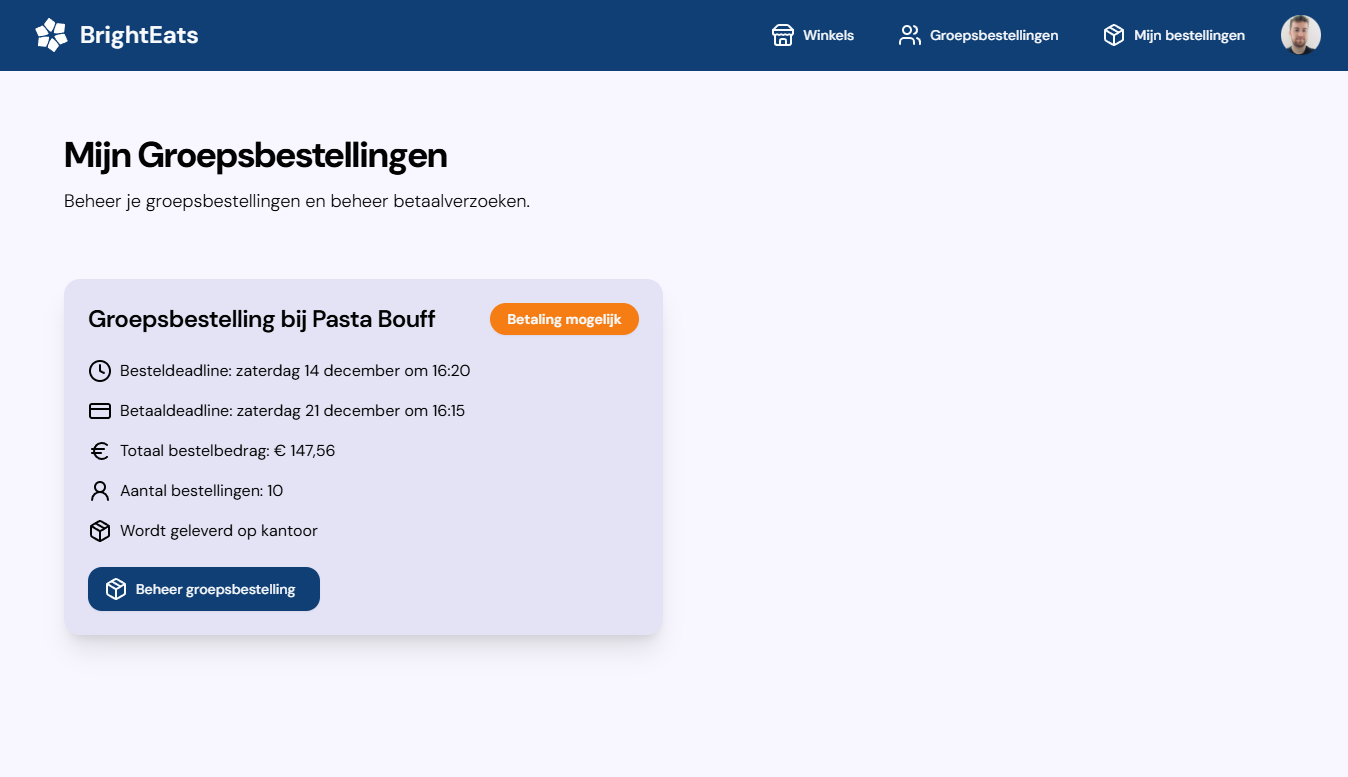
\includegraphics[width=0.8\textwidth]{my-group-orders-page.png}
\caption{Overzicht van group orders in de frontend}
\label{fig:group_orders_overview}
\end{figure}

\subsection{Conclusie}

De Vue.js frontend consumeert de \texttt{GroupOrder} resource via de \texttt{groupOrderService}, die de HTTP requests naar de API afhandelt. De TypeScript types in \texttt{types/group-order.ts} zorgen voor een duidelijke structuur van de data en maken type checking mogelijk. De componenten gebruiken de \texttt{groupOrderService} om data op te halen en te versturen, en verwerken de responses van de API. De conversiefuncties zorgen voor een correcte omzetting van het API formaat naar het frontend formaat.

Deze case study toont aan hoe de frontend en backend samenwerken om een consistente en gebruiksvriendelijke applicatie te realiseren. Door gebruik te maken van RESTful principes en een duidelijke structuur in zowel de frontend als de backend, wordt de ontwikkeling en het onderhoud van de applicatie simpel en efficiënt.

\section{OpenAPI}

Een belangrijk deel van onze RESTfulness guidelines is het gebruik van de OpenAPI-specificatie om de API te documenteren. Dit gaan we in deze sectie proberen te automatiseren. Er bestaan namelijk tools waarmee je de code van een Laravel-API automatisch kan omzetten naar een OpenAPI-specificatie. Wij gebruiken hiervoor de package \texttt{dedoc/scramble}.

\subsection{Problemen bij opzet}

Het opzetten van de documentatie was zeer simpel: we installeerden de package en stelden het configuratiebestand \texttt{scramble.php} in. Vervolgens starten we onze developmentomgeving en kregen we een mooie OpenAPI-specificatie te zien. Echter, bij het genereren van de specificatie van de Bright\-Eats API, liepen we tegen enkele problemen aan.

\bigskip

Ten eerste was de API-documentatie niet heel uitgebreid. De documentatie bevatte enkel de endpoints en de parameters, maar miste beschrijvingen, voorbeelden en een algemene structuur. Deze moesten we toevoegen door middel van PHPDoc comments in de controllers, requests en resources.

\bigskip

Ten tweede was er het probleem dat Policies nog niet ondersteund worden. Daardoor moesten we zelf een creatieve manier vinden om op een mooie manier een kopje 'Authorization' toe te voegen aan de documentatie. Dit hebben we gedaan door in de PHPDoc comments van de controllers met markdown een kopje `Authorization' toe te voegen.

\bigskip

Het resultaat mag er zijn: een draaiende documentatiewebsite met alle endpoints, resources, validatieregels, authorisatieregels, voorbeelden en zelfs een interactieve terminal waarmee rechtstreeks met de API kan worden gecommuniceerd.

\begin{figure}[H]
\centering
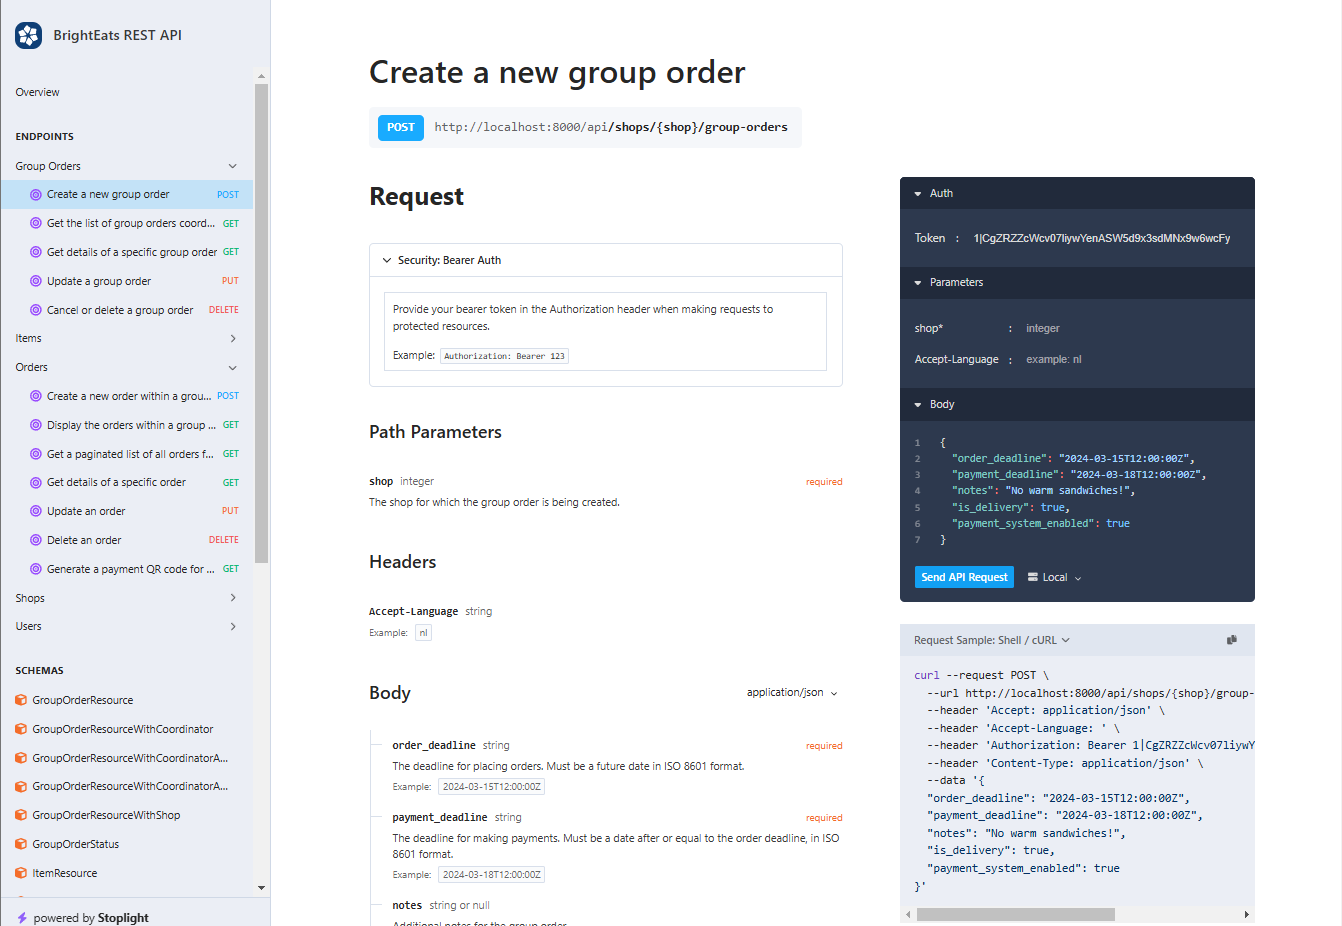
\includegraphics[width=0.8\textwidth]{scramble.png}
\caption{De OpenAPI documentatie van de Bright\-Eats API}
\label{fig:openapi}
\end{figure}

\subsection{Conclusie}

Het automatisch genereren van de OpenAPI-specificatie van een Laravel-API is een krachtige tool om de API te documenteren en te delen met andere ontwikkelaars. De \texttt{dedoc/scramble} package biedt een eenvoudige manier om de API-specificatie te genereren en te hosten. Door de documentatie te verrijken met PHPDoc comments en markdown, kan de documentatie nog verder worden verbeterd. Het resultaat is een gestructureerde en gedetailleerde documentatie van de API, die kan worden gebruikt om de API te begrijpen en te integreren in andere applicaties.

\section{Conclusie}

In dit hoofdstuk hebben we de implementatie van een RESTful API en frontend voor de Bright\-Eats applicatie besproken. We hebben de belangrijkste concepten en technieken behandeld die gebruikt zijn om een robuuste en schaalbare API te ontwikkelen. We hebben de structuur van de Laravel API en de Vue.js frontend besproken, en ook besproken hoe deze samenwerken om een volledige applicatie te vormen.

\bigskip

We hebben de implementatie van de \texttt{GroupOrder} resource in de backend en frontend geanalyseerd, en de verschillende onderdelen van de API en frontend besproken. We de controllers, services, modellen, API resources, requests, policies, Axios configuratie, API services, data types, en componenten die betrokken zijn bij het beheren van groepsbestellingen besproken.

\bigskip

Tot slot hebben we het genereren van de OpenAPI-specificatie voor de API met behulp van de \texttt{dedoc/scramble} package besproken. We hebben de uitdagingen en oplossingen besproken bij het documenteren van de API en het toevoegen van beschrijvingen, voorbeelden en authorisatieregels aan de documentatie.

\bigskip

De implementatie van de Bright\-Eats API en frontend illustreert hoe RESTful principes en best practices kunnen worden toegepast om een moderne en schaalbare applicatie te ontwikkelen. Door een duidelijke structuur en scheiding van verantwoordelijkheden te hanteren, wordt het onderhoud en de uitbreidbaarheid van de applicatie gegarandeerd. De documentatie van de API biedt een nuttige referentie voor het frontend team en andere ontwikkelaars die met de API willen integreren.
